\documentclass{article}

\usepackage{fancyhdr}
\usepackage{ragged2e}
\usepackage{graphicx}
\usepackage{caption}
\usepackage{geometry}
\usepackage{amsmath}
\usepackage{rotating}

\usepackage{listings}
\usepackage{color}

\definecolor{dkgreen}{rgb}{0,0.6,0}
\definecolor{gray}{rgb}{0.5,0.5,0.5}
\definecolor{mauve}{rgb}{0.58,0,0.82}

\lstset{frame=tb,
  language=Java,
  aboveskip=3mm,
  belowskip=3mm,
  showstringspaces=false,
  columns=flexible,
  basicstyle={\small\ttfamily},
  numbers=none,
  numberstyle=\tiny\color{gray},
  keywordstyle=\color{blue},
  commentstyle=\color{dkgreen},
  stringstyle=\color{mauve},
  breaklines=true,
  breakatwhitespace=true,
  tabsize=4
}

\setcounter{secnumdepth}{1}

\usepackage{chngcntr}
\counterwithin{figure}{section}

\renewcommand*{\thepage}{C\arabic{page}}

\pagestyle{fancy}
\lhead{ACME Robotics}
\chead{\#8367}
\rhead{\ifcontents Contents \else Week \thesection \fi}

\newif\ifcontents
\contentstrue

\makeatletter
\renewcommand{\@seccntformat}[1]{}
\makeatother

\begin{document}\contentsfalse


\subsection{Continue Developing The Team Marker}
%! Creating a releasing mechanism for the team marker. 
Shawn and Ben hadn't quite finished the anvil when they realized that the marker had no deployment mechanism and it looked super bad. They then decided to go with just a cube with a loop that could be dropped by a servo over the side. Shawn was tasked with making the block and he made it out of acrylic. Then Ben used basic Tetrix to make a servo mechanism that would unhook the cube and make it fall. Ben built the mechanism and found that a lot of servos didn't work.

\begin{figure}
    \centering
    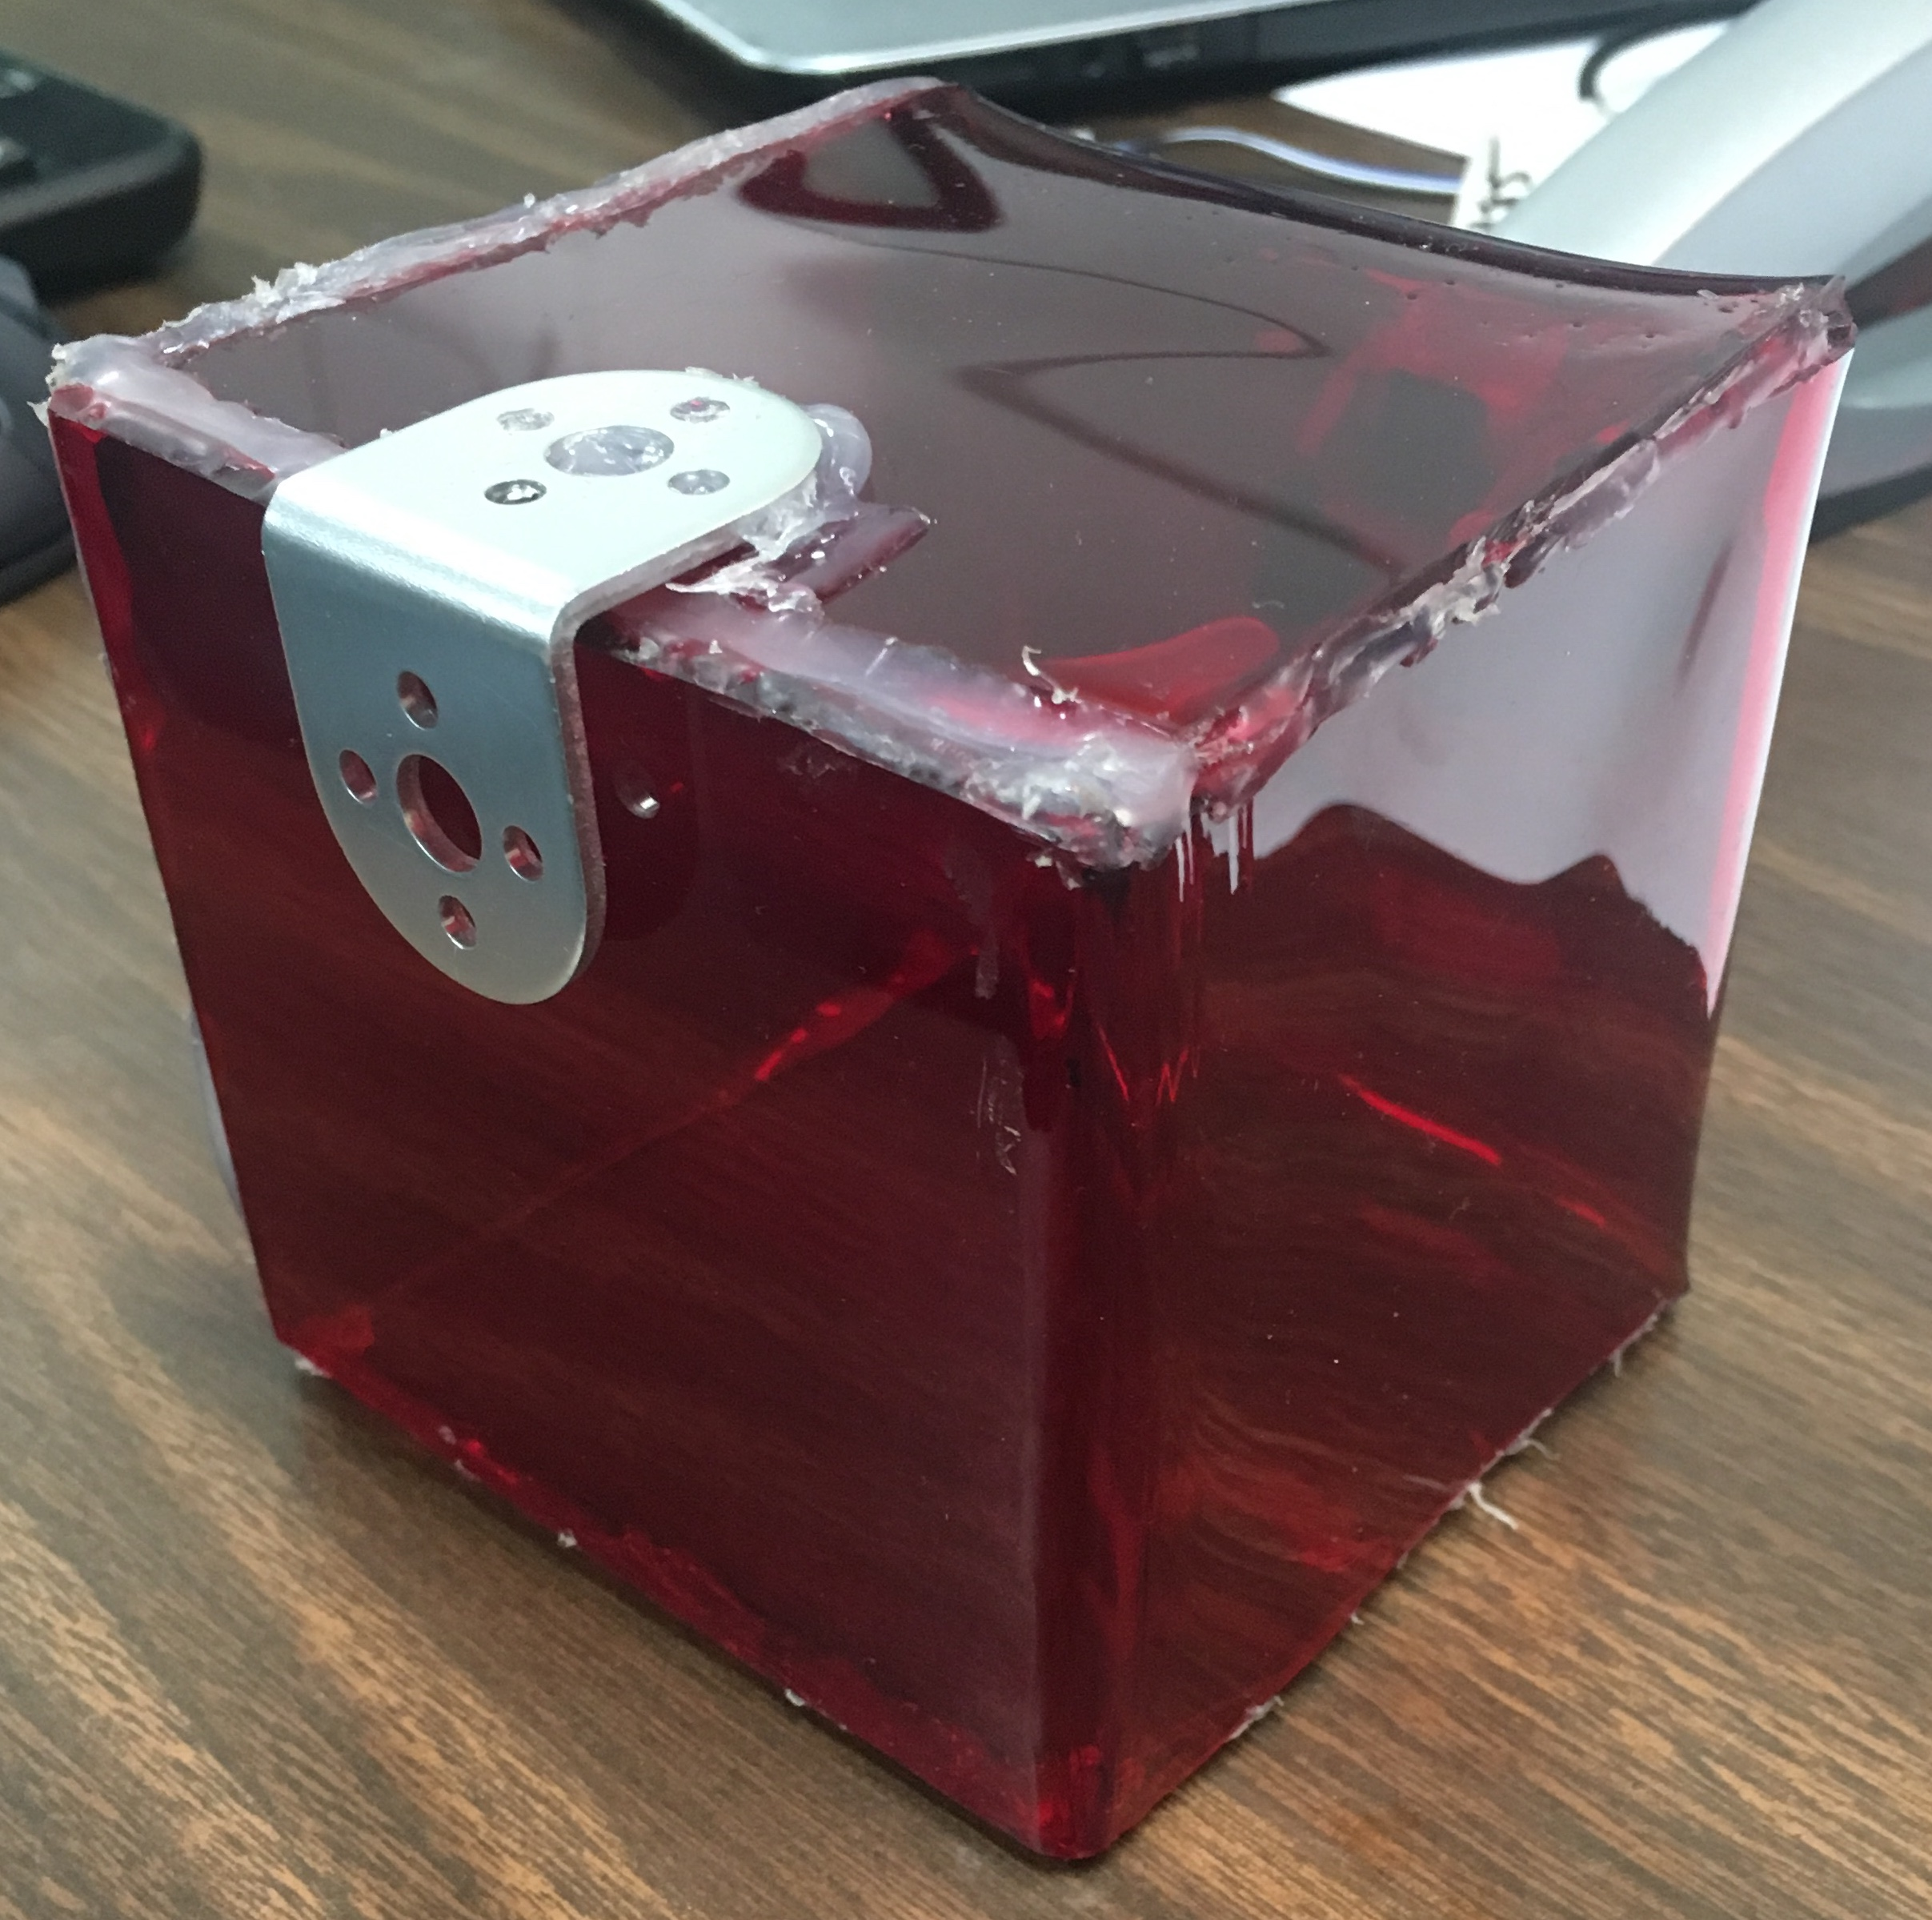
\includegraphics[width=.6\textwidth]{05_10-01/images/cube.jpg}
    \caption{Acrylic Cube}
    \label{fig:cube}
\end{figure}



\subsection{Drivetrain decision}
%! Decide on the design for the drivetrain.
The entire team made a matrix to help weight the pro and cons of the prototype drive-trains and already proven styles. The matrix took a lot in to consideration, such as agility, size, strength, traction, and maneuverability. The results of the matrix was a mecanum style drive-train driven by orbital 20 gearbox and belts. We choose this style because of its high speed, agility, and maneuverability, the downside to this style drive-train is the traction, which in turn can make playing defense a lot hard, compared to a none mecanum drive-train.  


\subsection{Develop X-rail based lift}
%! Draw a model of the x-rail based lift.
 After downloading all the required parts from Actobotics website and importing them into Inventor. He began assembling them per the design previously created. The first issue that had to be resolved was the mounting of the bearing bracket onto the x-rail. Because the maximum amount of space should be left on the inside of the lift, a mounting scheme other than the one suggested by Actobotics would have to be used. By swapping out the standoffs that came with the kit for shorter ones, the bearings could be brought closer to the x-rail they were attached to, reducing the spacing between stages to about a quarter inch. This reduced clearance between the stages necessitated another change. The default mounting hardware would fit, but as soon as bolts were added to the model the bolts would collide with the opposite rail. To resolve this, separate mounting hardware had to be found on the Actobotics website, allowing the bolts to clear each other. It would still be necessary to use lower profile 6-32 bolts than the standard Tetrix ones, but they should be able to be found at a hardware store. The inner carriage turned out to a be a little different than planned. There was no way to run more bearings along the front and back of the first stage box, because those grooves were already occupied by the bearings fixed to the top of the fixed stage. This meant that for the second stage to mount, a second piece of x-rail would have to be attached to the inside of the first piece, allowing the carriage to attach to it, or the carriage would have to run along the inside of the first stage. This would be possible with x-rail, because if the bearings pressed against the inside, the v-groves would prevent it from rotating forward and back, provided the top and bottom sets of bearings were spaced far enough apart to reduce the force applied laterally. This, however, would necessitate a different mounting strategy, because the brackets would have to attach to the end of the x-rail, rather than the sides. Unfortunately, the hole pattern on the end of the x-rail did not nicely match up with the hole pattern on the bracket, so Kelly decided to put two smaller vertical pieces of x-rail on either side of the cross-brace that would support the scoring mechanism, and then mount the bearings to that. 
 
 \begin{figure}
     \centering
     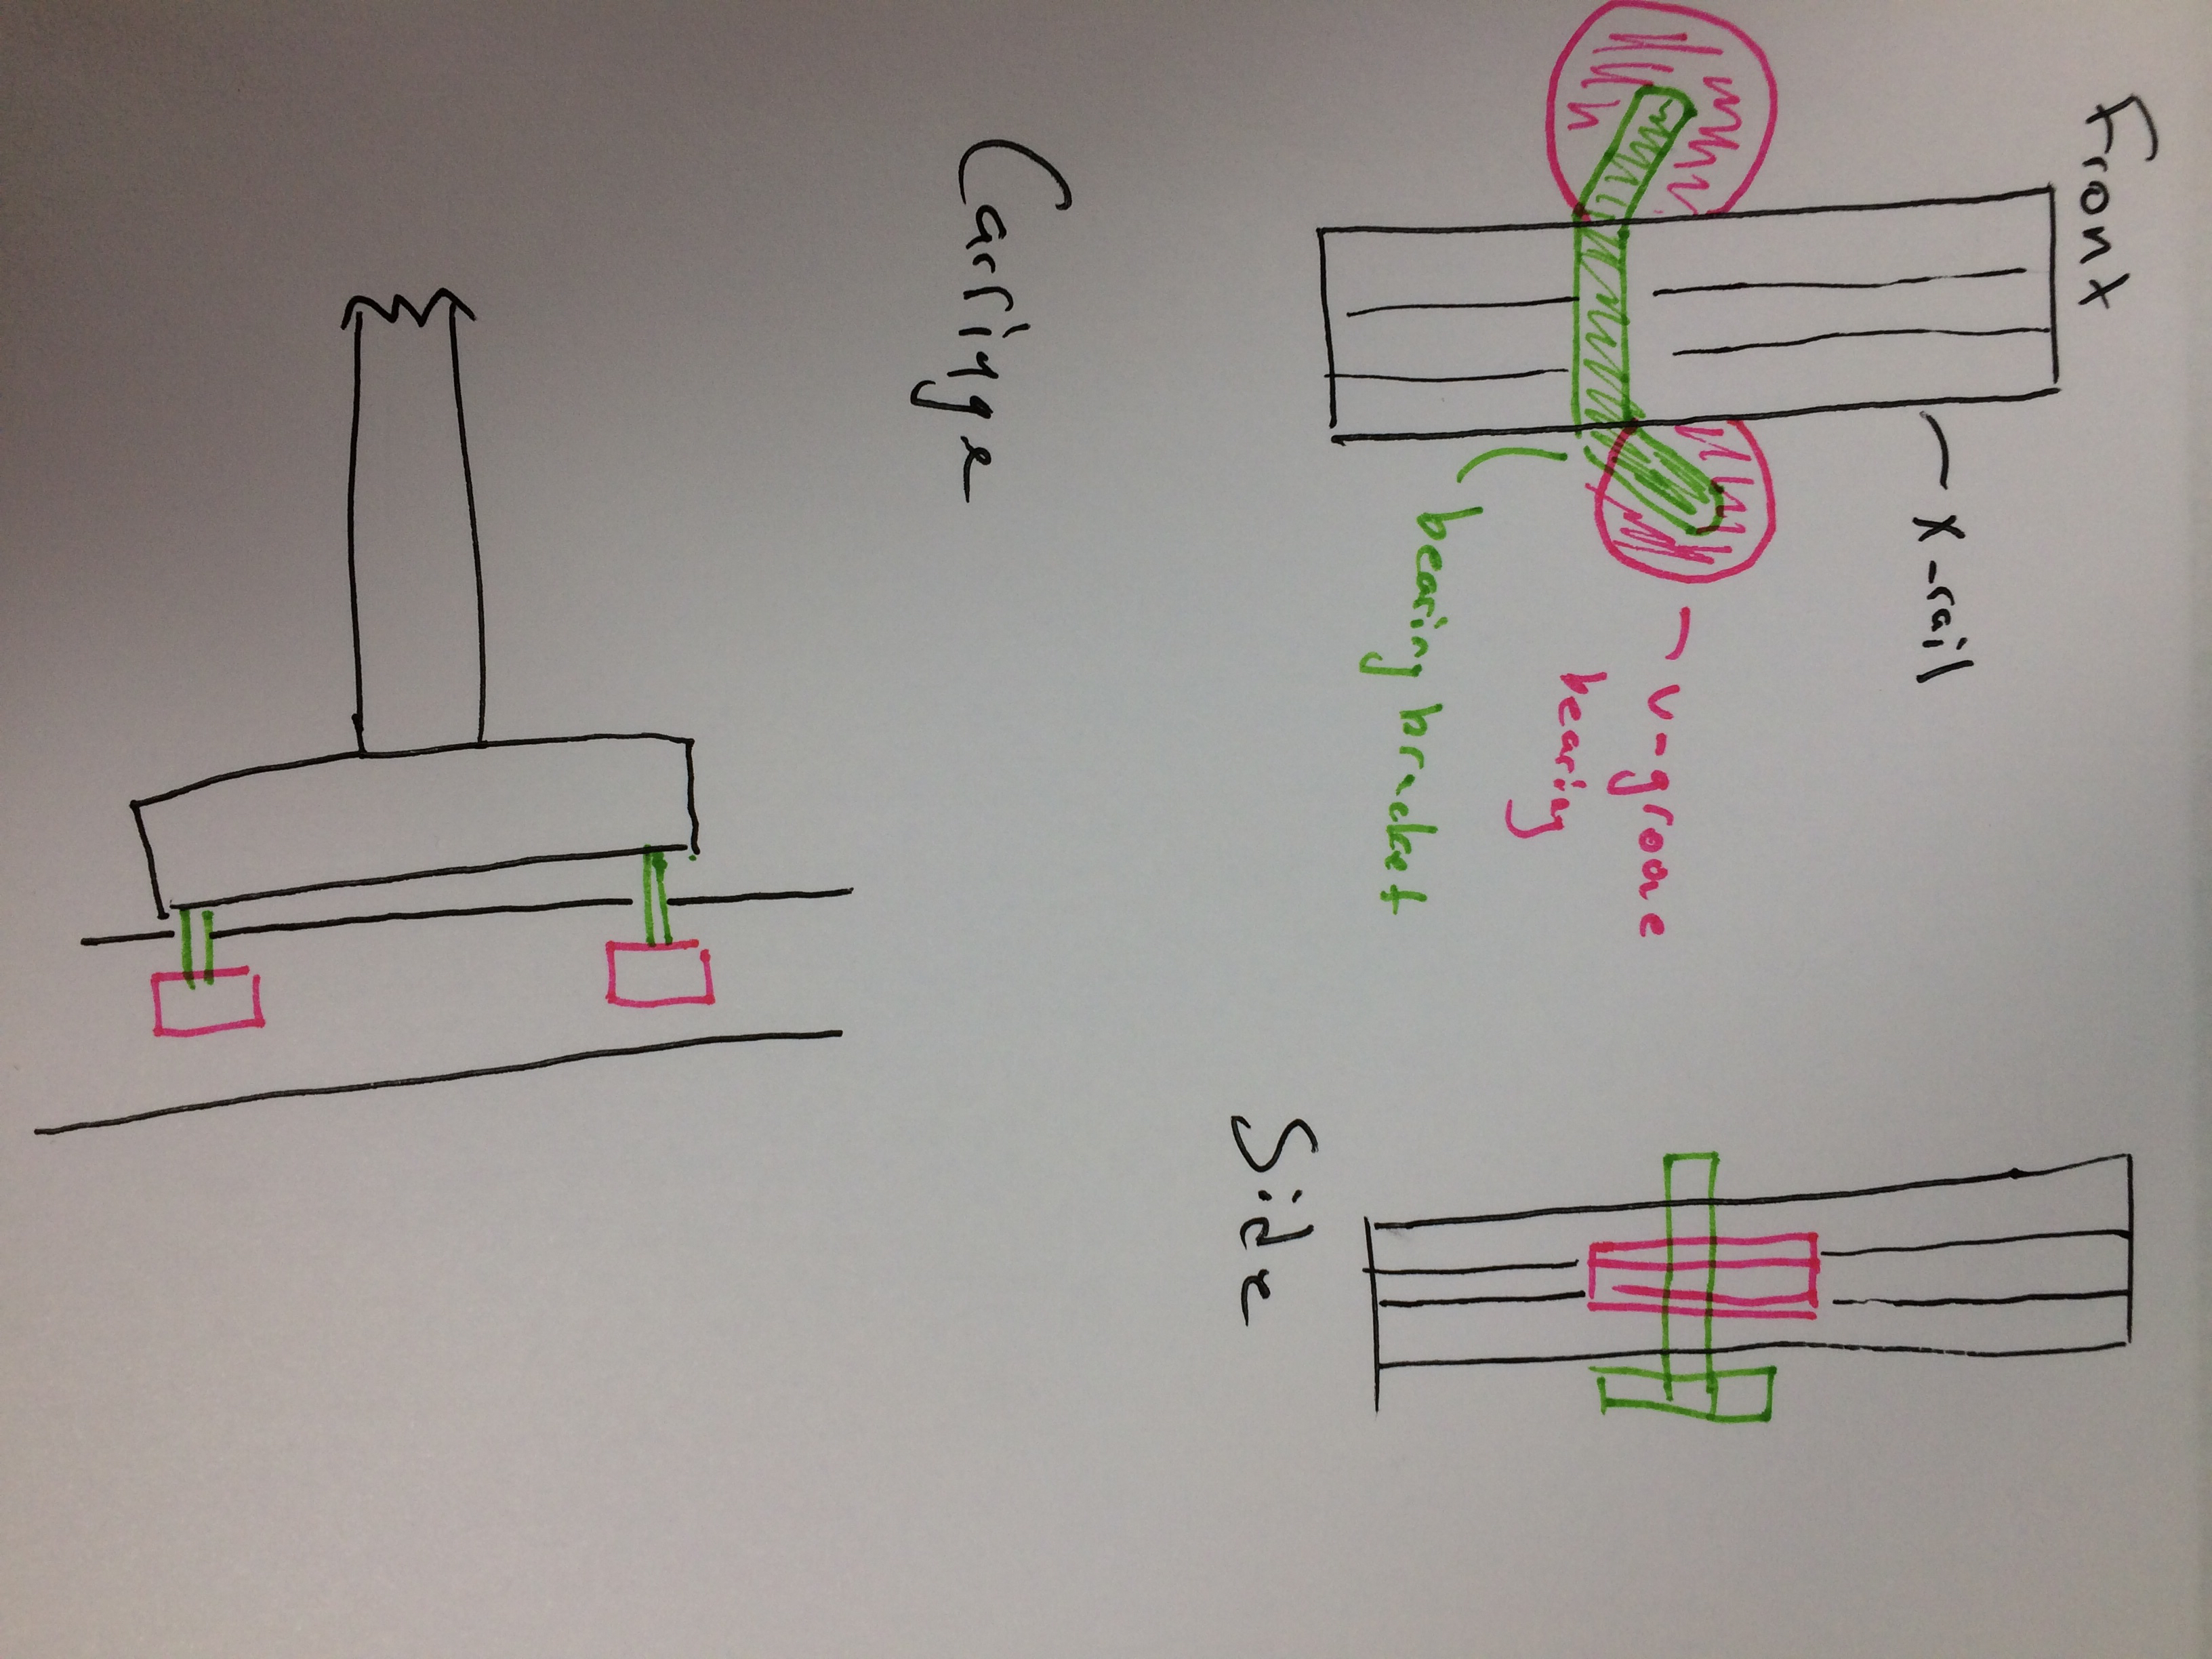
\includegraphics[width=.6\textwidth]{05_10-01/images/xrail.jpg}
     \caption{X-rail detail view}
     \label{fig:my_label}
 \end{figure}

\end{document}
